%!TEX program = xelatex
\documentclass[cn,hazy,black,10pt,normal]{elegantnote}
\usepackage{hyperref}
\usepackage{amssymb}
\usepackage{svg}

% font settings
\definecolor{mgreen}{RGB}{0,166,82}
\definecolor{guess}{RGB}{47,79,79}
\newenvironment{guess}{
  \color{guess}}{\newline \color{black}}

% cover settings
\title{数学作图测试}

\author{Johnny Tang}
\institute{DEEP Team}

\date{\zhtoday}

% customised commands

% 行距设置
\setlength{\lineskiplimit}{5pt} %至少宽度
\setlength{\lineskip}{4pt} %正常宽度
\setlength{\normallineskiplimit}{5pt} %正常宽度
\setlength{\normallineskip}{5pt} %正常宽度


\begin{document}

\maketitle

\chapter{Gnuplot作图实例}

万事开头难

\begin{lstlisting}
plot f(x) w l lc 'black' lw 2 dt '-.-' title 'new function'
# plot f(x) with line linecolor 'black' linewidth 2 dashtype '-.-' title 'new function'
\end{lstlisting}

\begin{figure}[h!]
	\centering
	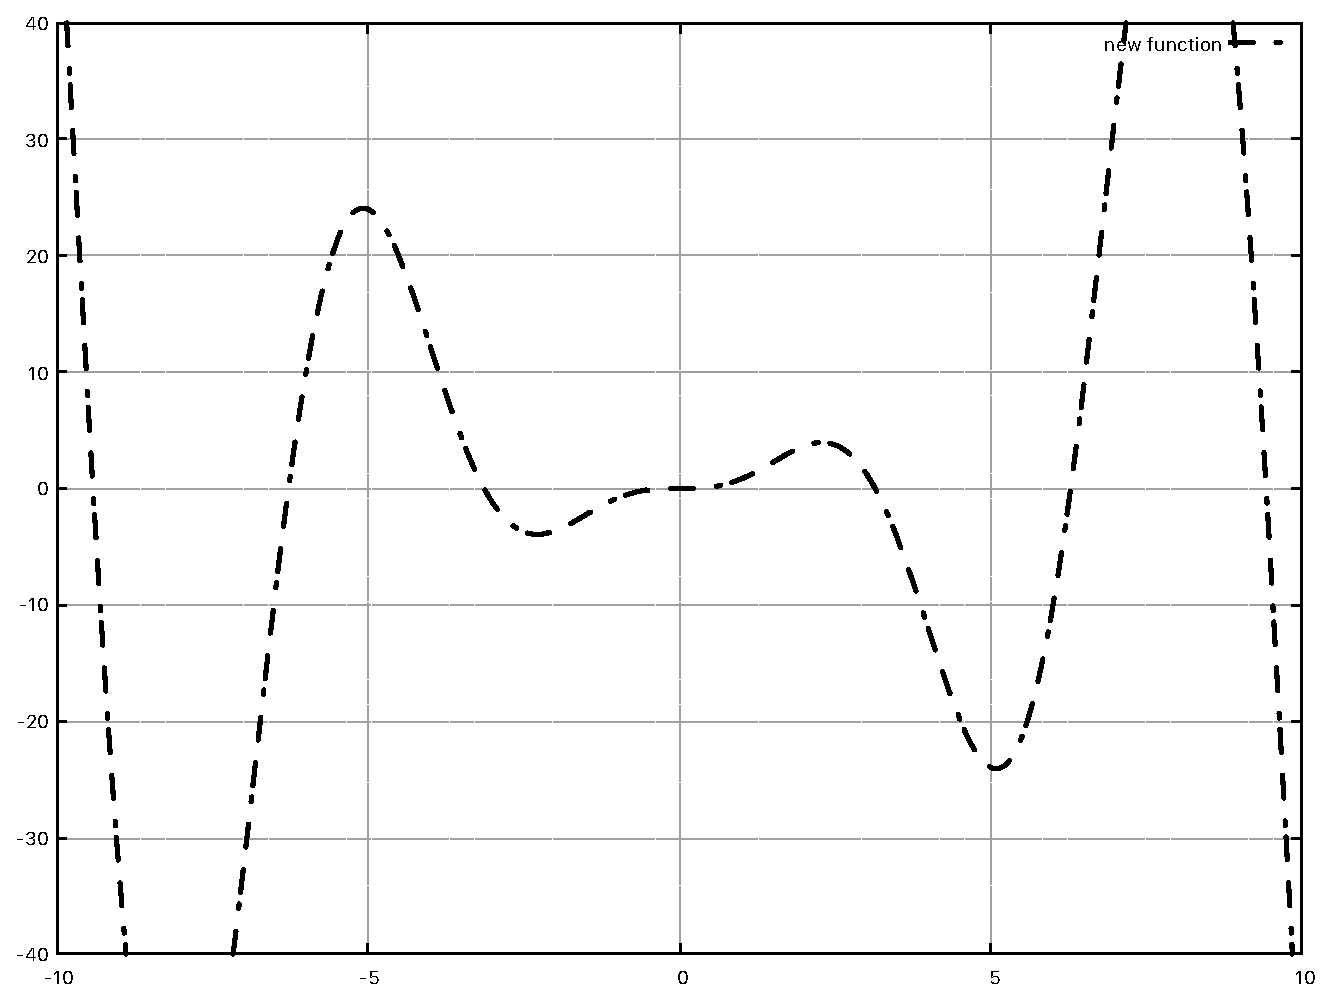
\includegraphics[width=12cm]{attachment/202304201.pdf}
	\caption{drawing a function}
\end{figure}

聚少成多

\begin{lstlisting}
#------------------------------Global Setting-------------------------#

set term svg font 'Times New Roman'
set encoding utf8
set encoding iso_8859_1

set size 0.9,0.8
set out 'example_plot1.svg'


#----------------------------------------------------------------------#

#-----------------------------Axes and frames--------------------------
unset border

xmin = -4
xmax = 4
ymin = -1
ymax = 4

set xzeroaxis linetype 1 lc 'black'
set yzeroaxis linetype 1 lc 'black'
set style arrow 3 head filled size screen 0.03,15,45 lc black
set arrow 1 from 0, 1.02*ymin to 0,1.05*ymax arrowstyle 3  
set arrow 2 from 1.02*xmin, 0 to 1.05*xmax,0 arrowstyle 3  

set xtics 1 nomirror axis
set ytics 1 nomirror axis #offset -0.5*(xmax - xmin),0
#unset xtics
#unset ytics
set mxtics 2
set mytics 2

#------------------------------------------------------------------

#--------------------------content setting------------------------
set xrange[xmin:xmax]
set yrange[ymin:ymax]
set samples 1000

f(x) = 2**x
g(x) = (1.0/2.0)**x
h(x) = 5**x
i(x) = (1.0/5.0)**x

#------------------------------------------------------------

#-----------------------------label setting---------------------
set xlabel '$x$'
set ylabel '$y$'
unset xlabel
unset ylabel
set label '{$x$}' at 1.05*xmax, 0.3 offset char 0, char 0 center font 'Times New Roman,22'
set label '{$y$}' at 0.3, 1.05*ymax offset char 0, char 0 center font 'Times New Roman,22'

set key top right
#---------------------------------------------------------------------


#-------------------------Start plotting---------------------------------------
plot f(x) lc 'red' lw 2, g(x) lc 'blue' lw 2, h(x) lc 'red' lw 2 dt '-', i(x) lc 'blue' lw 2 dt '-'

\end{lstlisting}

\begin{figure}[h!]
	\centering
	\includesvg[width=12cm]{gnuplot/example_plot1.svg}
	\caption{完整的作图示范}
\end{figure}

\begin{figure}[h!]
	\centering
	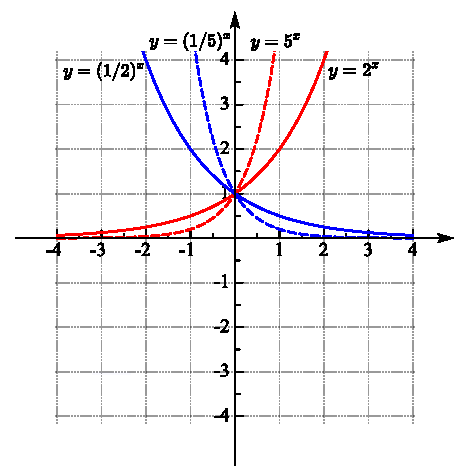
\includegraphics[width=12cm]{attachment/20230402viuuhjuu.pdf}
	\caption{相同的图像:与AxGlyph出图对比}
\end{figure}

\newpage
\section{预赛答案}

2022:

$\dfrac{38}{27}$;$-\dfrac{\sqrt{21}}{14}$;$32$;$[4-\sqrt{6},4)$;$288$;$\dfrac{\sqrt{7}}{4}$;$3$;$81$.

$y=2-\dfrac{x^2}{8}~(-4 \leq x \leq 4)$;$\dfrac{1}{2} \leq \lambda \leq 2$.

$a_n=1$.

略.

2021:

$-\dfrac{1}{4}$;$27$;$\dfrac{\sqrt{6}}{3}$;$3$;$[0,1]$;$2^{1011}$;$\dfrac{17}{21}$;$3816$.

$(x+1)^2+\dfrac{4}{3}y^2=1~(y \neq 0)$.

略.

$4$.



\end{document}
